\documentclass{article}

\usepackage{url} 

\usepackage{pdfpages}
\usepackage{lastpage}
\usepackage{fancyhdr}
\usepackage{ngerman}
\usepackage{listings}

\usepackage{floatrow}
\usepackage[tableposition=top]{caption}
\floatsetup[table]{capposition=top}

\usepackage{amsmath, amssymb}

\usepackage[utf8]{inputenc}


\usepackage[numbib]{tocbibind}



\newcommand\twodigits[1]{%
   \ifnum#1<10 0#1\else #1\fi
}



\lhead{Silbercoulombmeter}
\rhead{23. Oktober 2020\\T. Maier, J. Winkler}
%\cfoot{\twodigits{\thepage}~/ \pageref{LastPage}}
\cfoot{{\thepage}~/ \pageref{LastPage}}

\newcommand{\as}{\alpha_\text{spez}}

\begin{document}

\parindent0cm

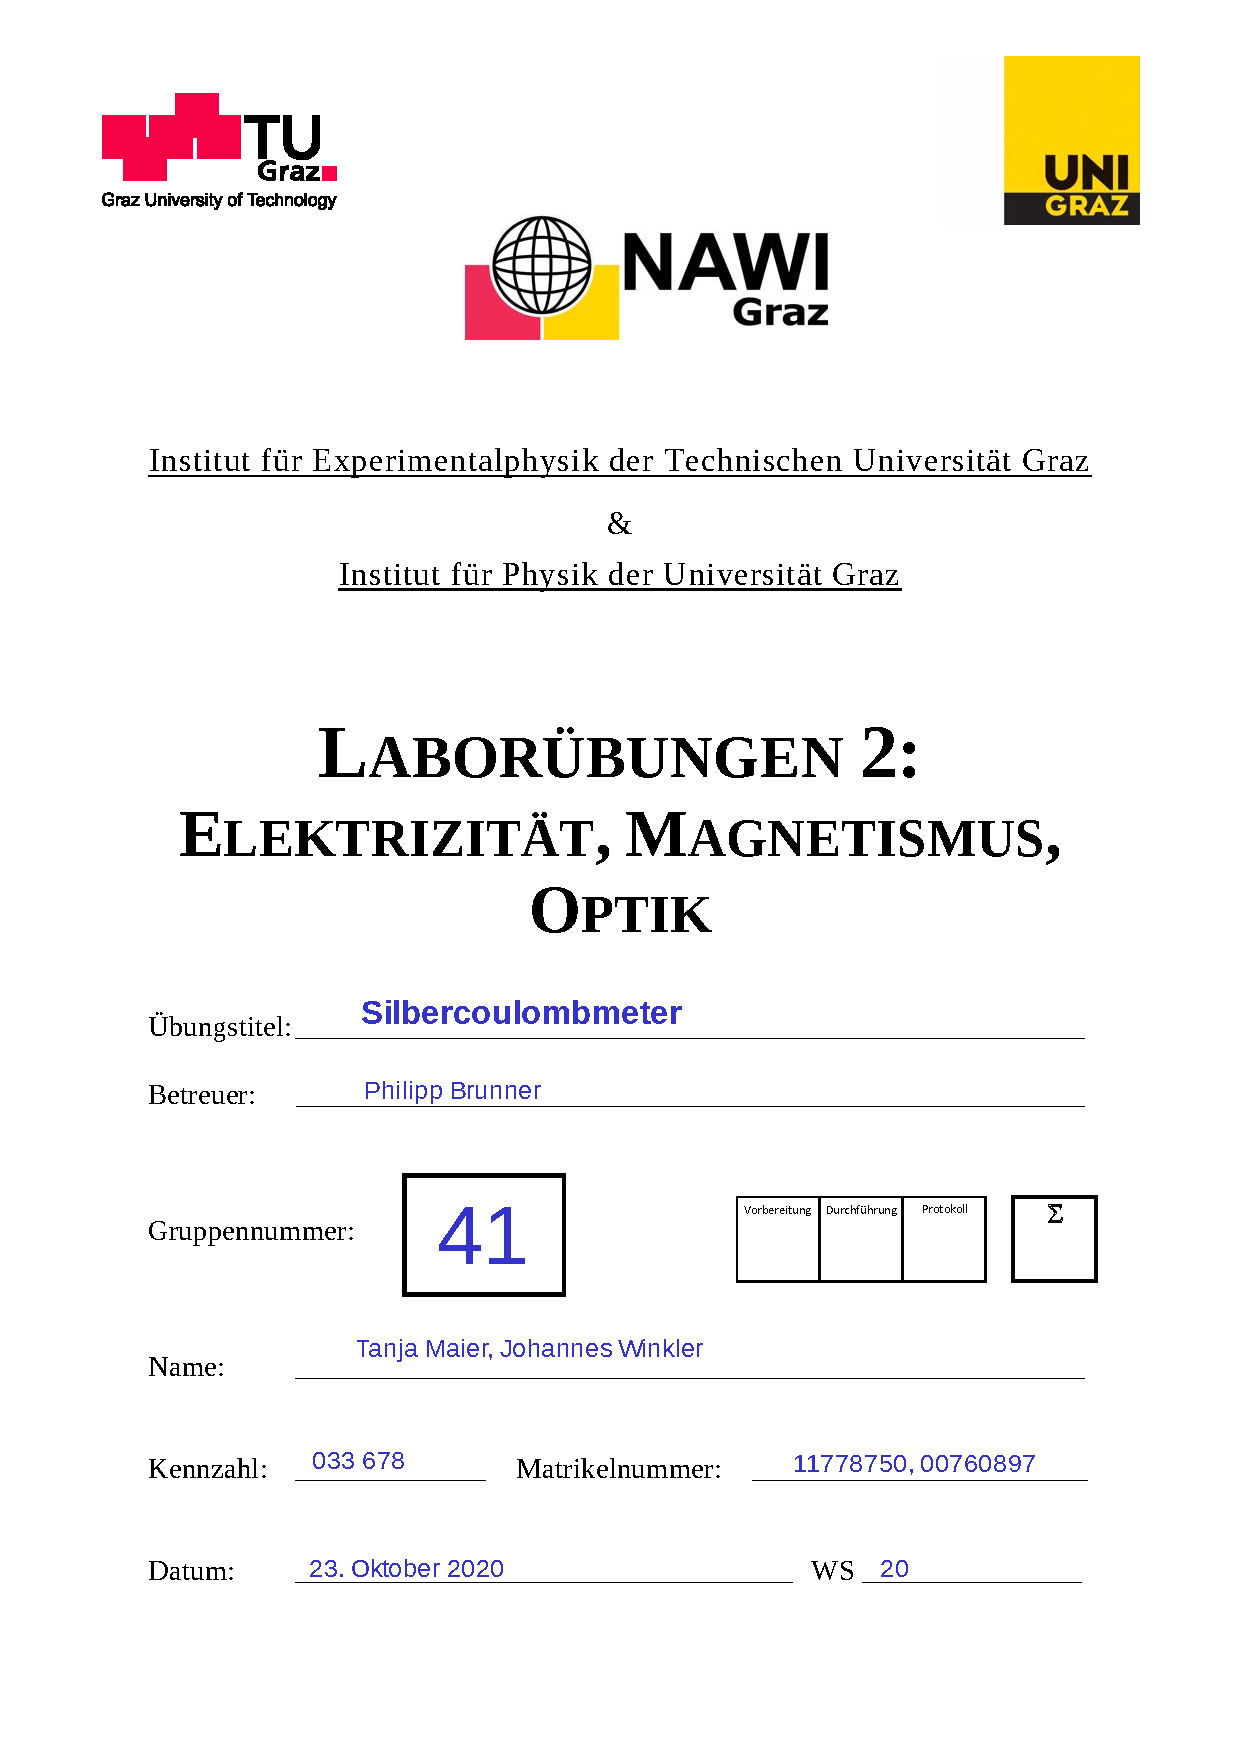
\includepdf{Deckblatt.pdf}


\pagestyle{fancy}

\section{Aufgabenstellung}






\section{Grundlagen und Versuchsaufbau}

Grundsätzlich versteht man unter Elektrolyse die Umwandlung von elektrischer Energie in chemische Energie. Atome bzw. Moleküle werden also mit Hilfe von Strom getrennt. Die Leitung in einem Elektrolyten erfolgt dabei über frei bewegliche Ionen im elektrischen Feld. Dabei entstehen durch Aufnahme von Elektroden der Kathode $z$-wertig positive Kationen oder Abgabe von Elektronen an die Anode z-wertig negative Anionen, wobei $z$ eine ganze Zahl ist.



\begin{figure}[H]
\caption{Ionentransport im Elektrolyten im elektrischen Feld. $A$ Anode, $K$ Kathode.}
\label{fig:pic1}
{\centering
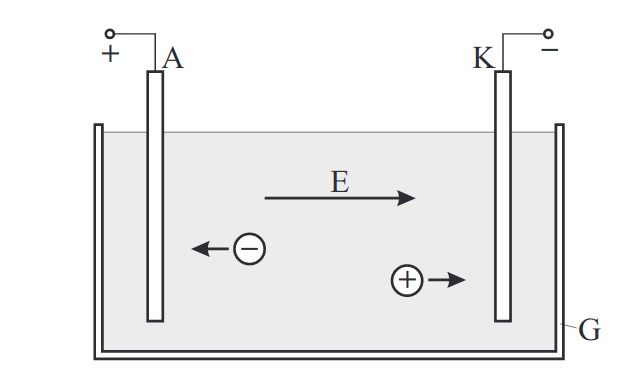
\includegraphics[scale=1.8]{pic1.png}}
\end{figure}

Bei einer Elektrolyse treten also an den beiden Elektroden chemische Vorgänge auf, da die Ionen des Elektrolyten auf Anode und Kathode reagieren. Dabei gilt
\begin{align}
q = n\cdot e \cdot z
\end{align}
wobei $n$ die Zahl der $z$-wertigen Ionen, $q$ die durch den Elektrolyten geflossene Elektrizitätsmenge und $e$ die Elementarladung ist.

Zur Bestimmung der Faraday-Konstante $F$ schickt man durch den Elektrolyten in einer Zeitspanne $t$ einen gemessenen Strom $I$ (und somit eine bekannte Elektrizitätsmenge $q$) und bestimmt die Menge $m$ eines an einer Elektrode abtransportierte Stoffmenge. Für ein z-wertiges Ion ergibt sich so das 1. Faraday'sche Gesetz
\begin{align}
q = I\cdot t = \frac{m}{M} \cdot F \cdot z
\end{align}



Die Stoffmenge der Elektrizitätsmenge durch einen Elektrolyten ist proportional zum Produkt von Stromstärke und Zeit.

Der Einfachheit wegen wählt man hierbei einen Elektrolyten, der ein stabiles Reaktionsprodukt ergibt, sodass durch Umformen leicht $F$ bestimmt werden kann. Umgekehrt kann man bei bekanntem $F$ auch leicht die Elektrizitätsmenge berechnen. Solche Apparaturen werden daher als Coulometer bezeichnet.

Unter Berücksichtigung des elektrochemischen Äquivalents $C$ (Stoffmenge, die bei der Elektrolyse mit einem Coulomb abgeschieden wird \cite{chemie}) gilt außerdem
\begin{align}
C = \frac{m_x}{z\cdot e} = \frac{m_x\cdot N_A}{z\cdot e \cdot N_A} = \frac{m_A}{z\cdot F}
\end{align}
Sowie auch das 2. Faraday'sche Gesetz: Die elektrochemischen Äquivalente zweier Stoffe verhalten sich gleich wie ihre chemischen Äquivalente.





\section{Geräteliste}

\begin{table}[H]
\caption{Liste der verwendeten Geräte}

~

\begin{tabular}{l|llll}
Bezeichnung & Hersteller & Gerätenummer & Unsicherheit \\
\hline
Thermometer & & & $\pm 1~^\circ$C \\
\end{tabular}

\end{table}




\section{Durchführung und Messwerte}

\subsection{Silbercoulombmeter}
Der Versuch wird gemäß Abbildung \ref{fig:pic1} aufgebaut. Die aus Silber bestehenden Elektroden werden abgeschliffen und ausführlich gewogen. Danach werden sie in den Behälter gehängt und an den Stromkreis angeschlossen. Es gilt $I=100~$mA für $t=1800~$s. Nach einer Stunde werden die Elektroden aus dem Behälter genommen und erneut abgewogen.


\subsection{Elektrolyse}


\section{Auswertung}

\subsection{Silbercoulombmeter}
Beim Silbercoulombmeter wird für die Faraday-Konstante folgende Formeln benötigt.
\begin{align*}
F &= \frac{I\cdot t\cdot M}{m\cdot z} \\
\Delta &= \frac{\Delta I\cdot t\cdot M}{m\cdot z} + \frac{I\cdot \Delta t\cdot M}{m\cdot z} +\frac{I\cdot t\cdot M}{m^2\cdot z}\cdot \Delta m
\end{align*}
Es gilt $z=1$ und $M=107.87~$g/mol laut \cite{silber}. Zusätzlich gilt $I=(100 \pm 2)~$mA und $t=(1800 \pm 1)~$s. Der Wert $m$ wird aus der Differenz der Elektroden abgelesen.

Für die Auswertung ergibt sich bei Tanja Maier
\begin{align*}
F_\text{Kathode} &= (94 \pm 47)~\text{kC/mol}\\
F_\text{Anode} &= (37 \pm 8)~\text{kC/mol} \\
e_\text{Kathode} &= (1.56 \pm 0.78)\cdot 10^{-19}~C \\
e_\text{Anode} &= (0.62 \pm 0.62)\cdot 10^{-19}~C  
\end{align*}

Bei den Messwerten von Johannes Winkler ergibt sich
\begin{align*}
F_\text{Kathode} &= (88 \pm 46)~\text{kC/mol}\\
F_\text{Anode} &= (127 \pm 91)~\text{kC/mol} \\
e_\text{Kathode} &= (1.5 \pm 0.8)\cdot 10^{-19}~C \\
e_\text{Anode} &= (2.1 \pm 2.1)\cdot 10^{-19}~C  
\end{align*}




\subsection{Elektrolyse}



\section{Zusammenfassung}




\section{Diskussion}





%\newpage 
%\appendix
%\section{Python Skript}



\definecolor{commentgreen}{RGB}{2,112,10}
\definecolor{eminence}{RGB}{108,48,130}
\definecolor{weborange}{RGB}{255,165,0}
\definecolor{frenchplum}{RGB}{129,20,83}

\lstdefinelanguage{python}{
    morekeywords={def, for, range, abs, return},
    otherkeywords={<-,->, |>, \%\{, \}, \{, \, (, )},
    sensitive=true,
    morecomment=[l]{\#},
    morecomment=[n]{/*}{*/},
    morecomment=[s][\color{purple}]{:}{\ },
    morestring=[s][\color{orange}]"",
    commentstyle=\color{commentgreen},
    keywordstyle=\color{eminence},
    stringstyle=\color{red},
	basicstyle=\ttfamily,
	breaklines,
	showstringspaces=false,
	frame=tb
}
%\lstinputlisting[language=Python,captionpos=b, label=lst:test,caption={Sinus Auswertung von Schaltung 1}]{analyse/analyse_ges.py}

%\lstinputlisting[language=Python,captionpos=b, label=lst:test,caption={Bessel Auswertung}]{generate_numbers_bessel.py}


%\lstinputlisting[language=Python,captionpos=b, label=lst:test,caption={Zerstreuungslinse Auswertung}]{generate_numbers_zerstreuungslinse.py}


\begin{thebibliography}{9}
\bibitem{chemie} \url{https://www.chemie.de/lexikon/Elektrochemisches_äquivalent.html}, 22.10.2020 22:53 Uhr
\bibitem{tu} bereitgestellte Unterlagen zum Versuch aus dem TeachCenter der TU Graz
\bibitem{silber} \url{https://de.wikipedia.org/wiki/Silber}, 25.10.2020, 11:35
\end{thebibliography}


\end{document}
